\section[TIỆM CẬN]{ĐƯỜNG TIỆM CẬN CỦA ĐỒ THỊ HÀM SỐ}
\subsection{TÓM TẮT LÝ THUYẾT}
\subsubsection{Đường tiệm cận ngang}%[Lý Văn Hoàng, Dự án TeX hóa Lý Thuyết]
\begin{dn}
    Đường thẳng $y=m$ là đường tiệm cận ngang (hay tiệm cận ngang)
    của đồ thị hàm số $y=f(x)$ nếu ít nhất một trong các điều kiện sau được thỏa mãn:\\
    \centerline{$\lim\limits_{x\to+\infty}f(x)=m, \quad\lim\limits_{x\to-\infty}f(x)=m $.}
\end{dn}
\begin{center}
    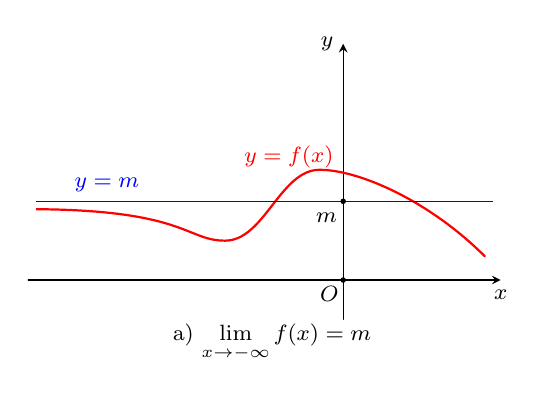
\begin{tikzpicture}[scale=1,>=stealth, font=\footnotesize, line join=round, line cap=round]
        \def\xmin{-4} \def\xmax{2}
        \def\ymin{-0.5} \def\ymax{3}
        %\draw[color=gray!50,dashed] (\xmin,\ymin) grid (\xmax,\ymax);
        \draw[->] (\xmin,0)--(\xmax,0) node [below]{$x$};
        \draw[->] (0,\ymin)--(0,\ymax) node [left]{$y$};
        \fill (0,0) circle (1pt) node[shift={(-135:2.5mm)}]{$O$};
        \node at (current bounding box.south) [below=-2pt] {a) $\lim\limits_{x \rightarrow-\infty} f(x)=m$};
        \clip (\xmin+0.1,\ymin+0.1) rectangle (\xmax-0.1,\ymax-0.1);
        \draw[red,thick,smooth,samples=300,domain=\xmin:\xmax]
        (-4,0.9)..controls +(0:2) and +(180:0.5)
        ..(-1.5,0.5)..controls +(0:0.5) and +(180:0.5)
        ..(-0.3,1.4)..controls +(0:0.5) and +(135:1)
        ..(1.8,0.3);
        \draw [blue](\xmin,1)--(\xmax,1);
        \path[blue] (-3,1)node[above]{$y=m$};
        \path[red] (0,1.3)node[above left]{$y=f(x)$};
        \fill (0,1) circle (1pt) node[shift={(-135:3mm)}]{$m$};
    \end{tikzpicture}\hspace*{1cm}
    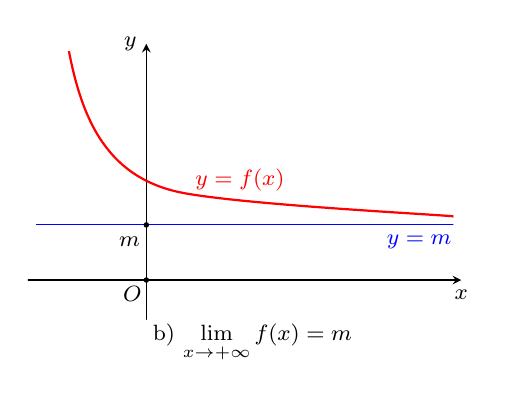
\begin{tikzpicture}[scale=1,>=stealth, font=\footnotesize, line join=round, line cap=round]
        \def\xmin{-1.5} \def\xmax{4}
        \def\ymin{-0.5} \def\ymax{3}
        %\draw[color=gray!50,dashed] (\xmin,\ymin) grid (\xmax,\ymax);
        \draw[->] (\xmin,0)--(\xmax,0) node [below]{$x$};
        \draw[->] (0,\ymin)--(0,\ymax) node [left]{$y$};
        \fill (0,0) circle (1pt) node[shift={(-135:2.5mm)}]{$O$};
        \node at (current bounding box.south) [below=-2pt] {b) $\lim\limits_{x \rightarrow+\infty} f(x)=m$};
        \clip (\xmin+0.1,\ymin+0.1) rectangle (\xmax-0.1,\ymax-0.1);
        \draw[red,thick,smooth,samples=300,domain=\xmin:\xmax]
        (-1,3)..controls +(-80:1) and +(170:1)
        ..(0.5,1.1)..controls +(170:-1) and +(180:-0.5)
        ..(3.9,0.8);
        \draw [blue](\xmin,0.7)--(\xmax,0.7);
        \path[blue] (4,0.7)node[below left]{$y=m$};
        \path[red] (0.5,1)node[above right]{$y=f(x)$};
        \fill (0,0.7) circle (1pt) node[shift={(-135:3mm)}]{$m$};
    \end{tikzpicture}
\end{center}
\begin{nx} \quad
    \begin{itemize}
        \item Để tìm tiệm cận ngang của đồ thị hàm số ta cần tính giới hạn của hàm số tại vô cực $(\pm \infty)$.
        \item Tìm giới hạn ở vô cực của hàm $y=\dfrac{P(x)}{Q(x)}$ với $P(x)$, $Q(x)$ là các đa thức không căn.
        \begin{enumerate}[i)]
            \item Bậc của $P(x)$ nhỏ hơn bậc của $Q(x) \Rightarrow \lim\limits_{x\to \pm\infty} y =0 \Rightarrow$ Tiệm cận ngang $Ox \colon y=0$.
            \item Bậc của $P(x)$ bằng bậc của $Q(x) \Rightarrow \lim\limits_{x\to \pm\infty} y = \dfrac{\text{Hệ số x bậc cao của P(x) }}{\text{Hệ số x bậc cao của Q(x)}} = \alpha$ (một số cụ thể) $\Rightarrow y= \alpha$ là tiệm cận ngang.
            \item Bậc của $P(x)$ lớn hơn bậc của $Q(x) \Rightarrow \lim\limits_{x\to \pm\infty} y = \pm \infty \Rightarrow$ Không có tiệm cận ngang.
        \end{enumerate}
    \end{itemize}
\end{nx}
\subsubsection{Đường tiệm cận đứng}%[Lý Văn Hoàng, Dự án TeX hóa Lý Thuyết]
\begin{dn}
    Đường thẳng $x=a$ được gọi là đường tiệm cận đứng (hay tiệm cận đứng) của đồ thị hàm số $y=f(x)$ nếu ít nhất một trong các điều kiện sau được thỏa mãn:
    $$ \lim\limits_{x \to a^{+} } f(x)= + \infty; \lim\limits_{x \to a^{+} } f(x)= - \infty ;$$ $$ \lim\limits_{x \to a^{-} } f(x)= + \infty; \lim\limits_{x \to a^{-}} f(x)= - \infty.$$
\end{dn}
\begin{center}
    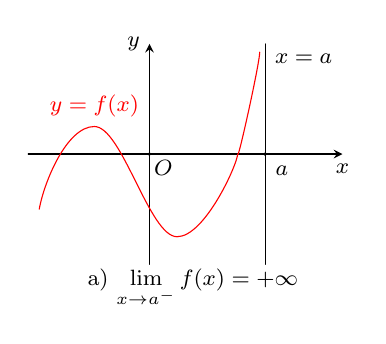
\begin{tikzpicture}[scale=.7,>=stealth, font=\footnotesize, line join=round, line cap=round]
        %Hình a
        \def\xmin{-2.2} \def\xmax{3.5}
        \def\ymin{-2} \def\ymax{2}
        %\draw[color=gray!50,dashed] (\xmin,\ymin) grid (\xmax,\ymax);
        \draw[->] (\xmin,0)--(\xmax,0) node [below]{$x$};
        \draw[->] (0,\ymin)--(0,\ymax) node [left]{$y$};
        \fill (0,0) circle (1pt) node[shift={(-45:2.5mm)}]{$O$};
        \draw (2.1,\ymin)--(2.1,\ymax)node[below right]{$x=a$};
        \fill (2.1,0) circle (1pt) node[shift={(-45:3mm)}]{$a$};
        %\clip (\xmin+0.1,\ymin+0.1) rectangle (\xmax-0.1,\ymax-0.1);
        \draw[red] (-2,-1)..controls +(80:0.5) and +(0:-.5)..(-1,0.5)node[above]{$y=f(x)$}
        ..controls +(0:0.5) and +(180:0.5)..(0.5,-1.5)
        ..controls +(0:0.5) and +(87:-0.2)..(1.6,0)
        ..controls +(87:-.2) and +(90:-0.2)
        ..(2,1.85);
        \node at (current bounding box.south) [below=-2pt] {a) $\lim\limits_{x \rightarrow a^{-}} f(x)=+\infty$};
    \end{tikzpicture}
    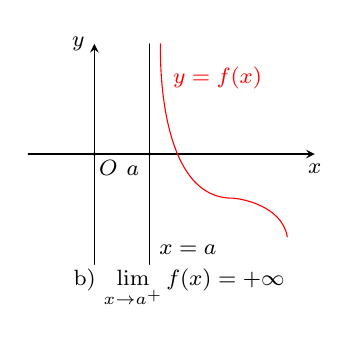
\begin{tikzpicture}[scale=.7,>=stealth, font=\footnotesize, line join=round, line cap=round]
        %Hình b
        \def\xmin{-1.2} \def\xmax{4}
        \def\ymin{-2} \def\ymax{2}
        %\draw[color=gray!50,dashed] (\xmin,\ymin) grid (\xmax,\ymax);
        \draw[->] (\xmin,0)--(\xmax,0) node [below]{$x$};
        \draw[->] (0,\ymin)--(0,\ymax) node [left]{$y$};
        \fill (0,0) circle (1pt) node[shift={(-45:2.5mm)}]{$O$};
        \draw (1,\ymin)node[above right]{$x=a$}--(1,\ymax);
        \fill (1,0) circle (1pt) node[shift={(-135:3mm)}]{$a$};
        \path[red] (1.25,1)node[above right]{$y=f(x)$};
        %\clip (\xmin+0.1,\ymin+0.1) rectangle (\xmax-0.1,\ymax-0.1);
        \draw[red] (1.2,2)..controls +(80:0) and +(0:-1.4)..(2.5,-0.8)
        ..controls +(0:0.1) and +(-80:-0.6)
        ..(3.5,-1.5);
        \node at (current bounding box.south) [below=-2pt] {b) $\lim\limits_{x \rightarrow a^{+}} f(x)=+\infty$};
    \end{tikzpicture}
    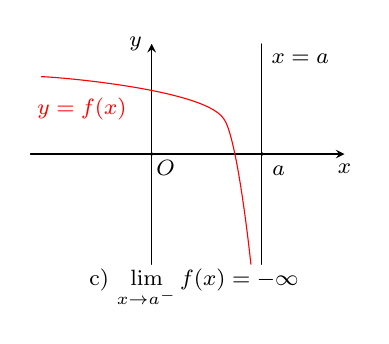
\begin{tikzpicture}[scale=.7,>=stealth, font=\footnotesize, line join=round, line cap=round]
        %Hình c
        \def\xmin{-2.2} \def\xmax{3.5}
        \def\ymin{-2} \def\ymax{2}
        %\draw[color=gray!50,dashed] (\xmin,\ymin) grid (\xmax,\ymax);
        \draw[->] (\xmin,0)--(\xmax,0) node [below]{$x$};
        \draw[->] (0,\ymin)--(0,\ymax) node [left]{$y$};
        \fill (0,0) circle (1pt) node[shift={(-45:2.5mm)}]{$O$};
        \draw (2,\ymin)--(2,\ymax)node[below right]{$x=a$};
        \fill (2,0) circle (1pt) node[shift={(-45:3mm)}]{$a$};
        \path[red] (-2.25,1.2)node[below right]{$y=f(x)$};
        %\clip (\xmin+0.1,\ymin+0.1) rectangle (\xmax-0.1,\ymax-0.1);
        \draw[red] (-2,1.4)..controls +(-10:-0.2) and +(-55:-.7)
        ..(1.3,0.65)..controls +(-50:0.4) and +(-90:0)
        ..(1.8,-2)
        ;
        \node at (current bounding box.south) [below=-2pt] {c) $\lim\limits_{x \rightarrow a^{-}} f(x)=-\infty$};
    \end{tikzpicture}
    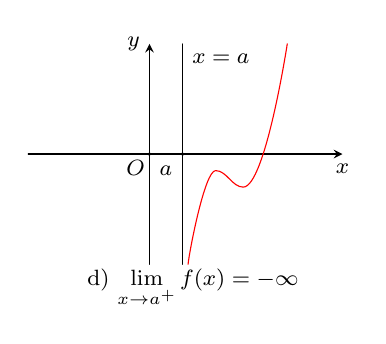
\begin{tikzpicture}[scale=.7,>=stealth, font=\footnotesize, line join=round, line cap=round]
        %Hình d
        \def\xmin{-2.2} \def\xmax{3.5}
        \def\ymin{-2} \def\ymax{2}
        %\draw[color=gray!50,dashed] (\xmin,\ymin) grid (\xmax,\ymax);
        \draw[->] (\xmin,0)--(\xmax,0) node [below]{$x$};
        \draw[->] (0,\ymin)--(0,\ymax) node [left]{$y$};
        \fill (0,0) circle (1pt) node[shift={(-135:2.5mm)}]{$O$};
        \draw (.6,\ymin)--(.6,\ymax)node[below right]{$x=a$};
        \fill (.6,0) circle (1pt) node[shift={(-135:3mm)}]{$a$};
        %\clip (\xmin+0.1,\ymin+0.1) rectangle (\xmax-0.1,\ymax-0.1);
        \draw[red] (0.7,-2)..controls +(85:0.2) and +(180:0.2)
        ..(1.2,-0.3)..controls +(0:0.2) and +(180:0.2)
        ..(1.7,-0.6)..controls +(0:0.4) and +(90:0)
        ..(2.5,2)
        ;
        \node at (current bounding box.south) [below=-2pt] {d) $\lim\limits_{x \rightarrow a^{+}} f(x)=-\infty$};
    \end{tikzpicture}
\end{center}
\immini{\textbf{Đặc biệt} Đối với hàm số $y= \dfrac{ax+b}{cx+d}$ có tiệm cận ngang $y=\dfrac{a}{c}$ và tiệm cận đứng $x= -\dfrac{d}{c}$. Tâm đối xứng là giao điểm của hai đường tiệm cận.
}{
    \begin{tikzpicture}[>=stealth, line join=round, line cap=round, font=\scriptsize,x=.8cm,y=.7cm]
        \begin{scope}[scale=.7]
            \def\a{1}
            \def\b{1}
            \def\c{1}
            \def\d{-2}
            \def\mau{red}
            \draw[->] (-5,0) -- (8,0) node[below] {$x$};
            \draw[->] (0,-5) -- (0,5) node[left] {$y$};
            \draw (0,0)node[below left]{$O$};
            \draw[dashed,blue] ({-\d/\c},-5)--({-\d/\c},5) (-5,{\a/\c})--(8,{\a/\c}); % Vẽ TCĐ và TCN
            \clip (-5,-5)rectangle(8,5);
            \draw ({-\d/\c},0)node[below right]{$2$};
            \draw (0,{\a/\c})node[above left]{$1$};
            \draw (7,-4)node[above left]{{\normalsize }$y=\dfrac{x+1}{x-2}$};
            \pgfmathsetmacro{\can}{-(\d)/(\c)}
            \draw[\mau,samples=150,smooth,domain=-5:{\can-.1}] plot(\x,{(\a*\x+(\b))/(\c*\x+(\d))}); % Vẽ nhánh bên trái TCĐ
            \draw[\mau,samples=150,smooth,domain={\can+.1}:8] plot(\x,{(\a*\x+(\b))/(\c*\x+(\d))}); % Vẽ nhánh bên phải TCĐ
        \end{scope}
\end{tikzpicture}}
\begin{nx} \quad
    \begin{itemize}
        \item Để tìm tiệm cận đứng của đồ thị hàm số, ta cần tính giới hạn một bên của $x_0$, với $x_0$ thường là điều kiện của hàm số (hay tại $x_0$ thì hàm số không xác định).
        \item Kỹ năng sử dụng máy tính (tham khảo):
        \begin{enumerate}[i)]
            \item Tính $\lim\limits_{x \to x_0^+} f(x)$ thì nhập $f(x)$ và CALC $x= x_0 + 10^{-9}$.
            \item Tính $\lim\limits_{x \to x_0^-} f(x)$ thì nhập $f(x)$ và CALC $x= x_0 - 10^{-9}$.
        \end{enumerate}
    \end{itemize}
\end{nx}
\subsubsection{Đường tiệm cận xiên}
\begin{dn}
    Đường thẳng $y=ax+b$ được gọi là đường tiệm cận xiên của đồ thị $(C):y=f(x)$ nếu \[\lim \limits_{x \to -\infty} \left[f(x)-(ax+b)\right]=0 \text{ hoặc }\lim \limits_{x \to +\infty} \left[f(x)-(ax+b)\right]=0\]
\end{dn}
\begin{center}
    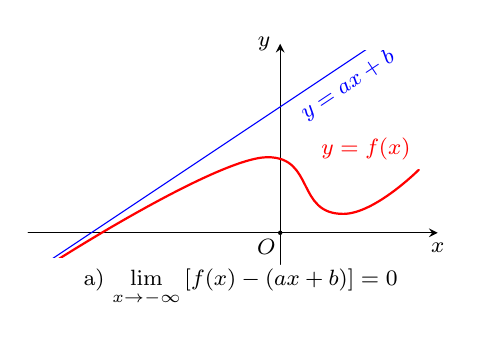
\begin{tikzpicture}[scale=0.8,>=stealth, font=\footnotesize, line join=round, line cap=round]
        \def\xmin{-4} \def\xmax{2.5}
        \def\ymin{-0.5} \def\ymax{3}
        %\draw[color=gray!50,dashed] (\xmin,\ymin) grid (\xmax,\ymax);
        \draw[->] (\xmin,0)--(\xmax,0) node [below]{$x$};
        \draw[->] (0,\ymin)--(0,\ymax) node [left]{$y$};
        \fill (0,0) circle (1pt) node[shift={(-135:2.5mm)}]{$O$};
        \node at (current bounding box.south) [below=-2pt] {a) $\lim\limits_{x \rightarrow-\infty}\left[f(x)-(ax+b)\right]=0$};
        \clip (\xmin+0.1,\ymin+0.1) rectangle (\xmax-0.1,\ymax-0.1);
        \draw[red,thick,smooth,samples=300,domain=\xmin:\xmax]
        (-3.8,-0.6)..controls +(34:0.5) and +(180:.75)
        ..(-0.2,1.2)..controls +(0:0.75) and +(180:.75)
        ..(1,0.3)..controls +(0:0.5) and +(80:0)
        ..(2.2,1);
        \draw[blue,smooth,samples=300,domain=\xmin:\xmax] plot(\x,{2/3*(\x)+2});
        \path[blue] (-3,0)--(0,2)node[below,sloped,pos=1.3]{$y=ax+b$};
        \path[red] (0.5,1)node[above right]{$y=f(x)$};
    \end{tikzpicture}\hspace{1cm}
    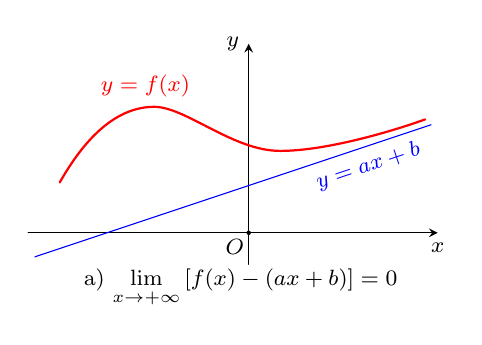
\begin{tikzpicture}[scale=0.8,>=stealth, font=\footnotesize, line join=round, line cap=round]
        \def\xmin{-3.5} \def\xmax{3}
        \def\ymin{-0.5} \def\ymax{3}
        %\draw[color=gray!50,dashed] (\xmin,\ymin) grid (\xmax,\ymax);
        \draw[->] (\xmin,0)--(\xmax,0) node [below]{$x$};
        \draw[->] (0,\ymin)--(0,\ymax) node [left]{$y$};
        \fill (0,0) circle (1pt) node[shift={(-135:2.5mm)}]{$O$};
        \node at (current bounding box.south) [below=-2pt] {a) $\lim\limits_{x \rightarrow+\infty}\left[f(x)-(ax+b)\right]=0$};
        \clip (\xmin+0.1,\ymin+0.1) rectangle (\xmax-0.1,\ymax-0.1);
        \draw[red,thick,smooth,samples=300,domain=\xmin:\xmax]
        (-3,0.8)..controls +(60:0.5) and +(180:.75)
        ..(-1.5,2)..controls +(0:.5) and +(180:.75)
        ..(0.5,1.3)..controls +(0:.75) and +(-160:.5)
        ..(2.8,1.8);
        \draw[blue,smooth,samples=300,domain=\xmin:\xmax] plot(\x,{1/3*(\x)+0.75});
        \path[blue] (-3,-0.25)--(0,0.75)node[below,sloped,pos=1.6]{$y=ax+b$};
        \path[red] (-2.5,2)node[above right]{$y=f(x)$};
    \end{tikzpicture}
\end{center}
\begin{nx}\quad
    \begin{itemize}
        \item Để tìm TCX của đồ thị hàm số $y=f(x)$ ta giải hệ phương trình: $\heva{& \lim \limits_{x \to +\infty} \dfrac{f(x)}{x}=a \ne 0 \\ & \lim \limits_{x \to +\infty} \left[f(x)-ax\right]=b}$ hoặc $\heva{& \lim \limits_{x \to -\infty} \dfrac{f(x)}{x}=a \ne 0 \\ & \lim \limits_{x \to -\infty} \left[f(x)-ax\right]=b}$, khi đó tiệm cận xiên của đồ thị hàm số $y=f(x)$ là đường thẳng $y=ax+b$.
        \item Đồ thị hàm số $y=\dfrac{mx^2+nx+p}{cx+d}=ax+b+\dfrac{r}{cx+d}$ có đường tiệm cận xiên là đường thẳng $y=ax+b$.
        \item Hàm phân thức có bậc tử bé hơn hoặc bằng bậc mẫu, bậc tử lớn hơn bậc mẫu 2 bậc thì không có tiệm cận xiên.
    \end{itemize}
\end{nx}